\documentclass[journal]{IEEEtran}
\usepackage{amsmath,amssymb,graphicx,booktabs,multirow,cite,hyperref,xcolor}

\begin{document}

\title{How Many Seeds Are Enough? A Reliability Audit and Seed-Count Guide for Deep RL Robot-Control Comparisons}

% Author information withheld for double-anonymous review, per RA-L submission
% instructions. Restore the \author{...} block with full name/affiliation/email
% for the camera-ready version after acceptance.
\author{\IEEEauthorblockN{Anonymous Author(s)}
\IEEEauthorblockA{Submitted for double-anonymous review}}

\markboth{Anonymous Submission}{Anonymous et al.: How Many Seeds Are Enough for Deep RL Robot-Control Comparisons?}

\maketitle

\begin{abstract}
Authors deciding how many random seeds to run, and reviewers judging a three-seed comparison
table, both need a concrete answer to the same question: how many seeds are actually enough? We
audit four algorithms (PPO, SAC, TD3, A2C) on four MuJoCo robot-control tasks with twenty seeds
each to provide one, comparing naive small-$N$ conclusions against a rigorous bootstrap analysis
(following Agarwal et al.) on the full data. For a genuine effect, a 3-seed study reaches the
wrong conclusion up to \input{tables/PILOT4_headline_worst_k3.tex}\% of the time; for the smallest
effect size we observe, this failure rate stays at 95\% even using nineteen of our twenty seeds,
and at the full twenty seeds a conventional Welch's $t$-test misses two such effects entirely
($p=0.060$ and $p=0.269$, on two different environments) that the rigorous method correctly
detects in both cases. We quantify these failure rates directly by exact combinatorial enumeration
of every $k$-seed sub-study ($k=3,\ldots,19$) drawable from our data, and explain the mechanism
with a statistical power analysis: the hardest case would need an estimated 126 seeds for
conventional 80\% power. From that analysis we build a general seed-count lookup table, keyed only
on observed effect size, that authors and reviewers can apply to their own comparisons without
rerunning our audit. We release our full pipeline, data, and code to support further audits.
\end{abstract}

\begin{IEEEkeywords}
Reinforcement learning, reproducibility, statistical power, robot control, benchmarking.
\end{IEEEkeywords}

\section{Introduction}

Deploying a learned policy on real hardware is normally preceded by a simulation stage that
selects which algorithm to use, and that selection is usually made from a handful of simulated
training seeds. This matters more in robotics than in RL generally: simulated seeds are
effectively free, but real-robot trials are not, they consume operator time, wear physical
hardware, and are frequently limited to single-digit repeats in
practice~\cite{mahmood2018benchmarking,dulac2021challenges}. If a simulated comparison with tens
of seeds is already unreliable, the same comparison run with the far smaller seed budgets
available on real hardware, or the sim-to-real pipelines that inherit a simulation-stage algorithm
choice~\cite{zhao2020simtoreal}, is likely worse, not better. Robot-control research increasingly
reports results produced by deep reinforcement learning (RL) policies, and papers introducing or
comparing such policies routinely support their claims with a small number of training seeds.
Henderson et al.~\cite{henderson2018deep} first documented how
sensitive deep RL results are to implementation details, hyperparameters, and random seed alone,
and argued that the small seed counts common in the literature at the time were inadequate to
support the significance claims being made. Colas et al.~\cite{colas2018many} formalized this
concern with a statistical power analysis, deriving, for a given effect size, how many seeds a
$t$-test or bootstrap comparison actually needs to reliably detect a true difference. Agarwal et
al.~\cite{agarwal2021deep} later proposed a suite of more statistically robust aggregate metrics,
stratified bootstrap confidence intervals and the interquartile mean (IQM) across runs and tasks,
as a replacement for point-estimate comparisons, packaged as the \texttt{rliable} library.

These works establish, from complementary angles, that naive small-$N$ significance testing in
deep RL is theoretically unreliable. What has been studied less is the direct, empirical question
a practitioner or reviewer actually faces: \emph{given the seeds a study happened to run, how
likely is it that its conclusion would have differed from a much larger, rigorous replication
of the same comparison?} This is a distinct question from power analysis in the abstract, because
it is conditioned on the actual, finite population of seeds a lab can afford to run, and it can be
answered directly, without additional assumptions, once a large enough reference sample has been
collected.

We provide that direct empirical answer for four algorithms — Proximal Policy Optimization
(PPO)~\cite{schulman2017proximal}, Soft Actor-Critic (SAC)~\cite{haarnoja2018soft}, Twin Delayed
DDPG (TD3)~\cite{fujimoto2018addressing}, and Advantage Actor-Critic
(A2C)~\cite{mnih2016asynchronous} — on four standard MuJoCo~\cite{todorov2012mujoco} continuous
control robot tasks, Reacher-v5, HalfCheetah-v5, Hopper-v5, and Walker2d-v5, implemented via
Stable-Baselines3 \cite{raffin2021stable} on Gymnasium~\cite{towers2024gymnasium}. Our contributions
are:

\begin{enumerate}
  \item A full statistical audit of \input{tables/PILOT4_n_runs.tex} independent training runs
    (twenty seeds per algorithm-environment pair), comparing naive Welch's $t$-tests, both
    uncorrected and Holm-corrected~\cite{holm1979sequentially} for multiple comparisons, against
    the rigorous bootstrap-CI'd probability of improvement from \texttt{rliable}.
  \item An exact combinatorial small-$N$ reliability analysis: for every algorithm pair and every
    $k \in \{3,\ldots,10,12,15,19\}$, we enumerate (or, where the combinatorial space is too large,
    densely sample) every possible $k$-seed sub-study drawable from our twenty seeds, and report the
    fraction that would have reached a conclusion contradicting the full-data answer.
  \item A statistical power analysis that explains this empirical result mechanistically, computing
    the power available at conventional seed counts (3, 5, 10) for each observed effect size, and
    the seed count that would be required for adequate (80\%) power.
  \item A general, audit-independent seed-count guide (Table~\ref{tab:seed_guide}): given an
    observed or pilot-estimated Cohen's $d$, the minimum seed count for 80\% or 90\% power under a
    two-sample $t$-test, usable directly by an author choosing how many seeds to run or a reviewer
    judging whether a reported seed count is adequate for the effect size being claimed.
  \item An open-source, reusable pipeline (training, statistical audit, small-$N$ reliability
    analysis, power analysis, and figure generation) that can be pointed at other algorithms,
    environments, or seed budgets to repeat this audit.
\end{enumerate}

\section{Related Work}

\textbf{Reproducibility in deep RL.} Henderson et al.~\cite{henderson2018deep} showed that
different random seeds, codebases, and even hyperparameter defaults can produce learning curves
that diverge as much as differences credited to genuine algorithmic improvements in the
literature, and recommended reporting more seeds together with appropriate uncertainty
quantification. Our work follows directly from their diagnosis, but asks the sharper question of
\emph{how large} the resulting risk of a wrong conclusion actually is, for realistic, currently-used
algorithms and tasks.

\textbf{Statistical power for RL comparisons.} Colas et al.~\cite{colas2018many} derived
closed-form and simulation-based power calculations for both the $t$-test and bootstrap
comparisons of RL algorithms, and is the most direct antecedent of our power analysis
(Section~\ref{sec:power}). Where their contribution is primarily theoretical and simulation-based
over synthetic effect sizes, we apply the same reasoning to effect sizes observed in real training
runs, and combine it with the empirical small-$N$ resampling result in
Section~\ref{sec:smalln}.

\textbf{Robust aggregate statistics.} Agarwal et al.~\cite{agarwal2021deep} introduced the
IQM-with-bootstrap-CI and probability-of-improvement metrics we adopt as our ``rigorous'' baseline
throughout this paper, and argued for their use across benchmark suites such as the Arcade
Learning Environment and Procgen. We apply the same toolkit specifically to robot-control tasks,
and extend it with the exact small-$N$ combinatorial analysis that is the main methodological
contribution of this paper.

\textbf{Real-world and sim-to-real RL.} Mahmood et al.~\cite{mahmood2018benchmarking} benchmark RL
algorithms directly on physical robots, at seed budgets orders of magnitude below simulation.
Dulac-Arnold et al.~\cite{dulac2021challenges} identify learning from limited real-system samples
as a core unsolved deployment challenge, and Zhao et al.~\cite{zhao2020simtoreal} survey the
sim-to-real pipelines through which a simulation-stage algorithm choice ultimately reaches physical
robots. Our audit quantifies a risk upstream of all three: an unreliable simulation-stage
comparison propagates into every downstream real-world or sim-to-real decision.

\section{Method}

\subsection{Experimental Setup}

We train four algorithms, PPO, SAC, TD3, and A2C, each with default Stable-Baselines3
hyperparameters and an MLP policy, on four continuous-control robot tasks from the Gymnasium MuJoCo
suite: Reacher-v5 (a low-dimensional, 10-observation/2-action reaching task) and three
progressively higher-dimensional locomotion tasks, HalfCheetah-v5 (17 observations, 6 actions),
Hopper-v5 (11 observations, 3 actions), and Walker2d-v5 (17 observations, 6 actions). Each
algorithm-task pair is trained for 200{,}000 timesteps, independently for twenty random seeds.
Every process is pinned to a single CPU thread
(\texttt{OMP\_NUM\_THREADS=1}, and equivalently for the other common BLAS thread-count
environment variables, plus \texttt{torch.set\_num\_threads(1)}) so that the many training runs
launched in parallel do not oversubscribe the host machine's CPU cores; without this, we observed
severe (multi-fold) slowdowns from thread contention. Final performance for each run is the mean
return over 30 deterministic evaluation episodes at the end of training. All 320 runs were trained
on a single CPU-only consumer machine (no GPU); the entire study, including the small-$N$ and
power analyses, required no specialized compute.

Observation normalization (running mean/variance, via \texttt{VecNormalize}) is applied
identically to all four algorithms during training, and reward normalization is applied during
training only, never at evaluation time, so reported returns remain on the environment's native
scale. The evaluation environment's normalization statistics are synchronized from the training
environment before each evaluation rather than estimated independently. This matters because
on-policy algorithms (PPO, A2C) are known to underperform off-policy algorithms (SAC, TD3) on
MuJoCo tasks for reasons traceable to such implementation details rather than the algorithms'
core update rules~\cite{engstrom2020implementation}; applying normalization uniformly avoids
confounding an implementation artifact with the genuine algorithmic and statistical questions this
audit is designed to answer.

\subsection{Rigorous Statistical Baseline}

For each algorithm on each environment, we report the interquartile mean (IQM, the mean after
discarding the top and bottom 25\% of runs) of the final evaluation return, with a 95\% confidence
interval from a percentile bootstrap (5{,}000 resamples) over the twenty seeds, following
\cite{agarwal2021deep}. For each pair of algorithms on each environment, we compute the rigorous
probability of improvement, $P(X > Y)$, the Mann-Whitney-based estimator of
\cite{agarwal2021deep}, together with its own bootstrap confidence interval; we call a pairwise
difference \emph{rigorously significant} when this CI excludes 0.5.

\subsection{Naive Baseline}

As a model of common current practice, we compute an uncorrected Welch's two-sample $t$-test on
the same seeds, and separately apply a Holm-Bonferroni correction~\cite{holm1979sequentially}
across the $\binom{4}{2}=6$ pairwise comparisons run within each environment, since a paper
comparing four algorithms typically runs multiple such tests without acknowledging the resulting
inflation of the family-wise error rate.

\subsection{Small-$N$ Reliability Analysis}
\label{sec:smalln}

The comparison above uses the same twenty seeds for both the naive and the rigorous methods, so it
tests only whether the choice of statistic matters, not whether the sample size does. The more
common failure mode described in \cite{henderson2018deep} and \cite{colas2018many} is that
published studies simply use far fewer seeds than we collected. We test this directly: for each
algorithm pair and each $k \in \{3, 4, \ldots, 10, 12, 15, 19\}$, we consider every way of choosing
$k$ of the twenty seeds for algorithm $A$ and $k$ of the twenty seeds for algorithm $B$ (an
exhaustive enumeration of $\binom{20}{k}^2$ sub-studies where this is computationally tractable,
and a dense random sample of up to 4{,}000 such sub-studies otherwise), run the naive $t$-test on
each, and record the fraction of sub-studies whose significance call disagrees with the rigorous,
full-$N$ answer. We separately record the fraction of \emph{directionally wrong} conclusions, cases where the small
sample not only differs in significance but asserts the opposite algorithm is better. Where the
sub-study space is too large for exact enumeration, we verified that the reported disagreement
rates are not an artifact of the sampling seed: repeating the analysis with an independent seed
changes any individual rate by at most 3.9 percentage points and by 0.24 on average.

\subsection{Power Analysis}
\label{sec:power}

To explain the small-$N$ reliability results mechanistically, we compute, for each algorithm
pair's empirically observed Cohen's $d$, the statistical power of a two-sample $t$-test at $n \in
\{3, 5, 8, 10, 15, 20, 30, 50\}$ seeds per arm, and the sample size required for conventional 80\%
power, using \texttt{statsmodels}. This connects the empirical disagreement rates of
Section~\ref{sec:smalln} to the underlying effect sizes driving them.

\section{Results}

\subsection{Per-Algorithm Performance}

Table~\ref{tab:iqm_summary} reports the IQM final return for each algorithm on each environment.

\begin{table}[t]
\centering
\footnotesize
\caption{Per-environment interquartile mean (IQM) final return with 95\% stratified bootstrap confidence intervals, by algorithm.}
\label{tab:iqm_summary}
\begin{tabular}{llrrr}
\toprule
Environment & Algo. & $n$ & IQM & 95\% CI \\
\midrule
Reacher-v5 & PPO & 20 & -4.80 & [-5.04, -4.56] \\
Reacher-v5 & SAC & 20 & -3.58 & [-3.73, -3.48] \\
Reacher-v5 & TD3 & 20 & -4.45 & [-4.69, -4.27] \\
Reacher-v5 & A2C & 20 & -11.69 & [-12.95, -10.48] \\
HalfCheetah-v5 & PPO & 20 & 1363.38 & [1298.71, 1519.46] \\
HalfCheetah-v5 & SAC & 20 & 7792.37 & [7259.68, 8263.73] \\
HalfCheetah-v5 & TD3 & 20 & 4529.14 & [2850.28, 6126.54] \\
HalfCheetah-v5 & A2C & 20 & 830.97 & [643.03, 1244.35] \\
Hopper-v5 & PPO & 20 & 1215.39 & [1032.53, 1915.02] \\
Hopper-v5 & SAC & 20 & 3147.32 & [2604.67, 3323.05] \\
Hopper-v5 & TD3 & 20 & 83.98 & [37.66, 425.71] \\
Hopper-v5 & A2C & 20 & 473.93 & [328.68, 722.20] \\
Walker2d-v5 & PPO & 20 & 741.90 & [680.15, 914.99] \\
Walker2d-v5 & SAC & 20 & 3974.62 & [3296.03, 4536.47] \\
Walker2d-v5 & TD3 & 20 & 1445.87 & [564.27, 2394.84] \\
Walker2d-v5 & A2C & 20 & 228.42 & [132.38, 330.53] \\
\bottomrule
\end{tabular}
\end{table}

Table~\ref{tab:aggregate} pools normalized scores across all four environments into a single
ranking, following the aggregate-metric methodology of \cite{agarwal2021deep}.

\begin{table}[t]
\centering
\footnotesize
\caption{Aggregate cross-environment ranking: IQM of min-max normalized scores pooled across all benchmark tasks, with 95\% bootstrap CI.}
\label{tab:aggregate}
\begin{tabular}{lrrr}
\toprule
Algorithm & $n$ scores & Normalized IQM & 95\% CI \\
\midrule
SAC & 80 & 0.886 & [0.834, 0.926] \\
TD3 & 80 & 0.419 & [0.289, 0.558] \\
PPO & 80 & 0.326 & [0.220, 0.467] \\
A2C & 80 & 0.130 & [0.093, 0.189] \\
\bottomrule
\end{tabular}
\end{table}

\subsection{Naive vs.\ Rigorous Significance}

Table~\ref{tab:pairwise} compares the naive (raw and Holm-corrected) and rigorous conclusions for
every algorithm pair, using the full twenty-seed sample, across all four environments. At full
sample size, the two methods disagree in 2/24 naive; 2/24 Holm-corrected of the
comparisons reported here. Twenty-two of the twenty-four comparisons are large enough effects that
both approaches agree they are real, but two are genuine disagreements even at $n=20$, one on each
of two independently trained environments. PPO versus TD3 on Reacher-v5: the naive Welch's
$t$-test narrowly misses significance ($p=0.060$), while the rigorous bootstrap-CI'd probability
of improvement correctly identifies the effect as real ($P(\text{TD3}>\text{PPO})=0.68$, 95\% CI
$[0.51, 0.84]$, excluding 0.5). A2C versus TD3 on Hopper-v5 is a starker version of the same
failure: the naive test is nowhere close to significance ($p=0.269$), while the rigorous method
again correctly detects a real effect ($P(\text{A2C}>\text{TD3})=0.77$, 95\% CI $[0.58, 0.92]$).
This is precisely the failure mode this paper is designed to surface: a real, modest effect that a
conventional significance test, even given a seed count several times larger than what most papers
report, fails to detect, while a more statistically efficient rigorous method resolves it
correctly. That this pattern recurs on a second, independently trained environment rules out the
possibility that the Reacher-v5 case was a one-off fluke of that particular task, and that these
are the \emph{only} two disagreements among twenty-four comparisons at full sample size also
confirms that, given twenty seeds, the choice of test statistic is a secondary source of
unreliability compared to sample size itself, which Section~\ref{sec:smalln} shows directly is the
dominant factor.

Neither disagreement is an artifact of one particular test choice, and the Hopper-v5 case has a
visible mechanistic cause. Thirteen of TD3's twenty seeds on Hopper-v5 collapse to a near-zero
return ($\le 38$), consistent with the training instability TD3 is known to exhibit on
Hopper-like tasks, while the remaining seeds succeed strongly (up to 2{,}888); A2C, in contrast,
never collapses, scoring between 55 and 2{,}732 on every seed. This bimodal failure pattern
inflates TD3's variance far beyond what a normal-theory test assumes, and that is exactly what
breaks a mean-based comparison: a rank-based Mann-Whitney $U$ test on the same data gives
$p=0.004$, correctly significant, while both the $t$-test and a distribution-free permutation test
on the mean difference ($p=0.29$) miss it. The Reacher-v5 disagreement has the same mechanism in
miniature: a rank-based Mann-Whitney $U$ test gives $p=0.047$ (correctly significant) and a
permutation test on the mean gives $p=0.060$ (matching the $t$-test's miss), because a single TD3
low-outlier run pulls the group mean without changing its rank. In both cases,
\texttt{rliable}'s probability-of-improvement estimator is itself a Mann-Whitney
statistic~\cite{agarwal2021deep}, so it inherits this same robustness. Naive practice defaults
almost universally to $t$-tests, so this is a realistic, not contrived, way for a real effect to
be missed, and the risk grows, not shrinks, whenever an off-policy algorithm's seed-to-seed
variance is inflated by occasional training failures, from a single low-outlier run (Reacher-v5)
to outright bimodal collapse in most seeds (Hopper-v5), both of which we observe from TD3 in this
data.

\begin{table*}[t]
\centering
\footnotesize
\caption{Pairwise algorithm comparisons: naive Welch's $t$-test (raw and Holm-corrected) versus the rigorous bootstrap-CI'd probability of improvement, on the full seed set. A ``significant'' rigorous call means the 95\% CI on $P(A>B)$ excludes 0.5.}
\label{tab:pairwise}
\begin{tabular}{llrrccccc}
\toprule
Env. & Pair ($A$ vs $B$) & $n_A$ & $n_B$ & Naive $p$ & Naive sig.\ & Holm sig.\ & $P(A{>}B)$ [95\% CI] & Rigorous sig.\ \\
\midrule
Reacher-v5 & A2C vs PPO & 20 & 20 & 4.2e-09 & \checkmark & \checkmark & 0.00 [0.000, 0.000] & \checkmark \\
Reacher-v5 & A2C vs SAC & 20 & 20 & 4e-10 & \checkmark & \checkmark & 0.00 [0.000, 0.000] & \checkmark \\
Reacher-v5 & A2C vs TD3 & 20 & 20 & 2.3e-09 & \checkmark & \checkmark & 0.00 [0.000, 0.000] & \checkmark \\
Reacher-v5 & PPO vs SAC & 20 & 20 & 7.3e-12 & \checkmark & \checkmark & 0.01 [0.000, 0.030] & \checkmark \\
Reacher-v5 & PPO vs TD3 & 20 & 20 & 0.06 & -- & -- & 0.32 [0.158, 0.495] & \checkmark \\
Reacher-v5 & SAC vs TD3 & 20 & 20 & 3.3e-09 & \checkmark & \checkmark & 0.98 [0.950, 1.000] & \checkmark \\
HalfCheetah-v5 & A2C vs PPO & 20 & 20 & 0.026 & \checkmark & \checkmark & 0.23 [0.075, 0.410] & \checkmark \\
HalfCheetah-v5 & A2C vs SAC & 20 & 20 & 1.2e-25 & \checkmark & \checkmark & 0.00 [0.000, 0.000] & \checkmark \\
HalfCheetah-v5 & A2C vs TD3 & 20 & 20 & 1.3e-06 & \checkmark & \checkmark & 0.07 [0.015, 0.168] & \checkmark \\
HalfCheetah-v5 & PPO vs SAC & 20 & 20 & 2.9e-21 & \checkmark & \checkmark & 0.00 [0.000, 0.000] & \checkmark \\
HalfCheetah-v5 & PPO vs TD3 & 20 & 20 & 7.9e-06 & \checkmark & \checkmark & 0.04 [0.003, 0.110] & \checkmark \\
HalfCheetah-v5 & SAC vs TD3 & 20 & 20 & 3.7e-06 & \checkmark & \checkmark & 0.93 [0.832, 0.985] & \checkmark \\
Hopper-v5 & A2C vs PPO & 20 & 20 & 0.00027 & \checkmark & \checkmark & 0.11 [0.025, 0.225] & \checkmark \\
Hopper-v5 & A2C vs SAC & 20 & 20 & 2.6e-12 & \checkmark & \checkmark & 0.01 [0.000, 0.060] & \checkmark \\
Hopper-v5 & A2C vs TD3 & 20 & 20 & 0.27 & -- & -- & 0.77 [0.580, 0.917] & \checkmark \\
Hopper-v5 & PPO vs SAC & 20 & 20 & 4e-05 & \checkmark & \checkmark & 0.15 [0.043, 0.292] & \checkmark \\
Hopper-v5 & PPO vs TD3 & 20 & 20 & 3.2e-05 & \checkmark & \checkmark & 0.91 [0.795, 0.985] & \checkmark \\
Hopper-v5 & SAC vs TD3 & 20 & 20 & 6.5e-13 & \checkmark & \checkmark & 0.98 [0.940, 1.000] & \checkmark \\
Walker2d-v5 & A2C vs PPO & 20 & 20 & 0.00011 & \checkmark & \checkmark & 0.01 [0.000, 0.022] & \checkmark \\
Walker2d-v5 & A2C vs SAC & 20 & 20 & 5e-11 & \checkmark & \checkmark & 0.00 [0.000, 0.000] & \checkmark \\
Walker2d-v5 & A2C vs TD3 & 20 & 20 & 0.00012 & \checkmark & \checkmark & 0.12 [0.035, 0.230] & \checkmark \\
Walker2d-v5 & PPO vs SAC & 20 & 20 & 3.8e-10 & \checkmark & \checkmark & 0.02 [0.000, 0.065] & \checkmark \\
Walker2d-v5 & PPO vs TD3 & 20 & 20 & 0.057 & -- & -- & 0.50 [0.285, 0.695] & -- \\
Walker2d-v5 & SAC vs TD3 & 20 & 20 & 5.6e-07 & \checkmark & \checkmark & 0.90 [0.802, 0.978] & \checkmark \\
\bottomrule
\end{tabular}
\end{table*}

\subsection{Small-$N$ Reliability}

Figure~\ref{fig:smalln} and Table~\ref{tab:smalln} show, for every algorithm pair, how the
disagreement rate against the full-data conclusion falls as the number of seeds $k$ used in the
hypothetical small study increases. At $n=20$, twenty-three of the twenty-four algorithm pairs we
test show a genuine effect (Section~\ref{sec:power_results} discusses the exception), so
disagreement in this analysis is almost entirely driven by false negatives: the naive test usually
detects the effect's correct direction whenever it finds significance at all, but at $k=3$ it
frequently fails to detect the effect in the first place. We did observe a small number of
\emph{directionally wrong} conclusions, at most 0.175\% of sub-studies for any single (pair, $k$)
combination, confirming that outright sign errors are rare but not strictly impossible even for
these effect sizes.

The three smallest observed effect sizes in the entire dataset (Section~\ref{sec:power_results})
are exactly the three pairs that are hardest to resolve here, a clean correspondence between
effect size and small-$N$ reliability that holds across all four environments. A2C vs.\ TD3 on
Hopper-v5, our smallest effect size, disagrees with the full-data conclusion in 93.7\% of possible
3-seed sub-studies, and the rate barely falls as $k$ grows: it is still wrong 95.0\% of the time at
$k=19$, using every seed but one of our full budget. PPO vs.\ TD3 on Reacher-v5, the next-smallest
effect, disagrees in 92.7\% of 3-seed sub-studies, falling only to 74.0\% by $k=19$. A2C vs.\ PPO on
HalfCheetah-v5, the fourth-smallest effect, shows the same pattern less severely, falling from
83.2\% at $k=3$ to 11.3\% at $k=19$. All three trace directly back to their small effect sizes: a
modest true difference does not become easy to detect just because more seeds are available, it
requires substantially more, and Hopper-v5's A2C vs.\ TD3 case shows this can mean \emph{almost no
seed count in practical use resolves it at all}.

The third-smallest effect size, PPO vs.\ TD3 on Walker2d-v5, is qualitatively different: it does
not reach significance under either method even at our full $n=20$ (Section~\ref{sec:power_results}),
so ``disagreement'' here means a $k$-seed sub-study claiming significance that the full,
still-underpowered sample does not support, rather than a sub-study missing a confirmed effect.
Counter-intuitively, this rate \emph{rises} with $k$, from 8.3\% at $k=3$ to 41.5\% at $k=19$,
because as $k$ approaches our full budget a sub-study's power approaches whatever partial power our
own $n=20$ study has for this effect (48.8\%, Table~\ref{tab:power}), so it announces significance
about as often as chance and available power together allow. This is a reminder that our
reliability metric is defined relative to the full-data answer, and when that answer is itself an
inconclusive, underpowered non-result, the disagreement rate does not behave the same way it does
for a confirmed genuine effect.

The remaining twenty pairs, all with larger effect sizes, show the more familiar and reassuring
pattern: high disagreement at $k=3$ that falls to single digits within a few more seeds and to zero
well before $k=19$.

\begin{figure}[t]
  \centering
  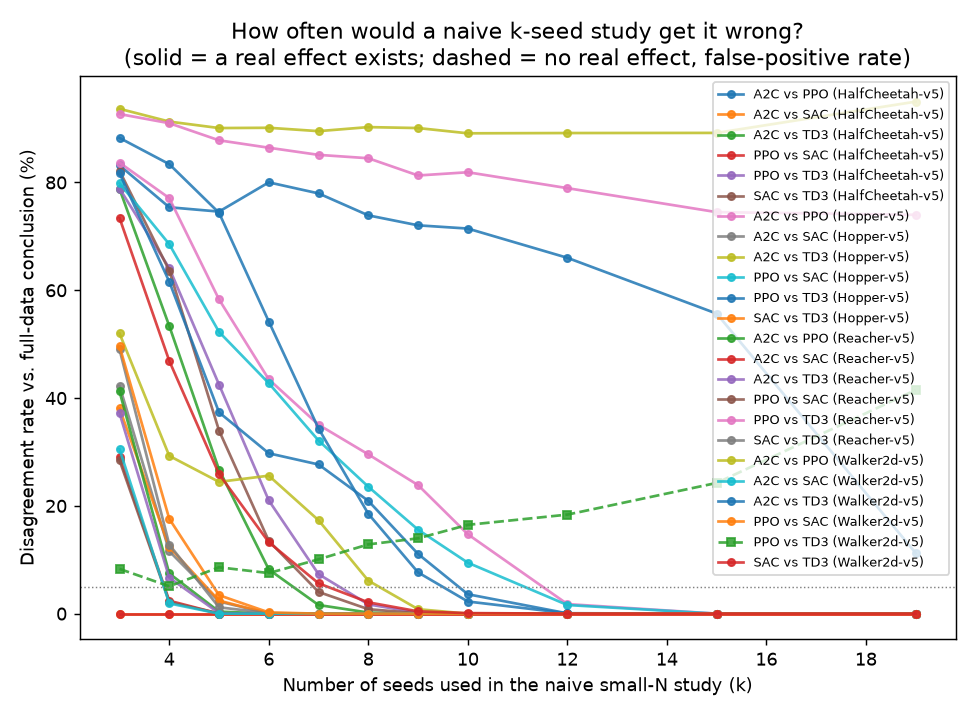
\includegraphics[width=\linewidth]{../figures/smalln_disagreement_PILOT4.png}
  \caption{Disagreement rate between a naive $k$-seed study and the full-data (twenty-seed) rigorous
  conclusion, as a function of $k$, for every algorithm pair across all four environments. All but
  one of the twenty-four pairs shown have a genuine effect at full sample size; the exception, PPO
  vs.\ TD3 on Walker2d-v5, remains inconclusive under both methods (Section~\ref{sec:power_results}).
  The two pairs that stay wrong even at large $k$ (A2C vs.\ TD3 on Hopper-v5, PPO vs.\ TD3 on
  Reacher-v5) are exactly the two smallest confirmed effect sizes.}
  \label{fig:smalln}
\end{figure}

\begin{table*}[t]
\centering
\footnotesize
\caption{Small-$N$ reliability at $k=3$ seeds: probability that a naive 3-seed study reaches a conclusion that disagrees with the full-data rigorous answer, computed by exact (or, where noted, sampled) enumeration of 3-seed subsets. The full $k=3,\ldots,19$ sweep for every pair is released with our data and plotted in Fig.~\ref{fig:smalln}.}
\label{tab:smalln}
\begin{tabular}{llcrrr}
\toprule
Env. & Pair & Real effect? & Trials & \% naive sig.\ & Disagreement rate \\
\midrule
HalfCheetah-v5 & A2C vs PPO & \checkmark & 4000 & 16.8\% & 83.2\% \\
HalfCheetah-v5 & A2C vs SAC & \checkmark & 4000 & 100.0\% & 0.0\% \\
HalfCheetah-v5 & A2C vs TD3 & \checkmark & 4000 & 21.2\% & 78.8\% \\
HalfCheetah-v5 & PPO vs SAC & \checkmark & 4000 & 100.0\% & 0.0\% \\
HalfCheetah-v5 & PPO vs TD3 & \checkmark & 4000 & 21.1\% & 78.9\% \\
HalfCheetah-v5 & SAC vs TD3 & \checkmark & 4000 & 17.8\% & 82.2\% \\
Hopper-v5 & A2C vs PPO & \checkmark & 4000 & 16.3\% & 83.7\% \\
Hopper-v5 & A2C vs SAC & \checkmark & 4000 & 57.8\% & 42.2\% \\
Hopper-v5 & A2C vs TD3 & \checkmark & 4000 & 6.3\% & 93.7\% \\
Hopper-v5 & PPO vs SAC & \checkmark & 4000 & 20.1\% & 79.8\% \\
Hopper-v5 & PPO vs TD3 & \checkmark & 4000 & 18.3\% & 81.7\% \\
Hopper-v5 & SAC vs TD3 & \checkmark & 4000 & 61.9\% & 38.1\% \\
Reacher-v5 & A2C vs PPO & \checkmark & 4000 & 58.8\% & 41.2\% \\
Reacher-v5 & A2C vs SAC & \checkmark & 4000 & 70.9\% & 29.1\% \\
Reacher-v5 & A2C vs TD3 & \checkmark & 4000 & 62.8\% & 37.2\% \\
Reacher-v5 & PPO vs SAC & \checkmark & 4000 & 71.5\% & 28.4\% \\
Reacher-v5 & PPO vs TD3 & \checkmark & 4000 & 7.3\% & 92.7\% \\
Reacher-v5 & SAC vs TD3 & \checkmark & 4000 & 51.0\% & 49.0\% \\
Walker2d-v5 & A2C vs PPO & \checkmark & 4000 & 48.0\% & 52.0\% \\
Walker2d-v5 & A2C vs SAC & \checkmark & 4000 & 69.5\% & 30.5\% \\
Walker2d-v5 & A2C vs TD3 & \checkmark & 4000 & 11.7\% & 88.3\% \\
Walker2d-v5 & PPO vs SAC & \checkmark & 4000 & 50.4\% & 49.6\% \\
Walker2d-v5 & PPO vs TD3 & -- & 4000 & 8.3\% & 8.3\% \\
Walker2d-v5 & SAC vs TD3 & \checkmark & 4000 & 26.6\% & 73.4\% \\
\bottomrule
\end{tabular}
\end{table*}

\subsection{Why Small Samples Fail: Power Analysis}
\label{sec:power_results}

Figure~\ref{fig:power} and Table~\ref{tab:power} show the statistical-power explanation for the
above: several algorithm pairs have effect sizes so large (Cohen's $d > 3$) that even $n=3$ seeds
gives reasonable power, while the three persistently hard-to-detect pairs identified above have
small-to-medium effect sizes for which even our full $n=20$ sample is underpowered. A2C vs.\ TD3 on
Hopper-v5 has $d=0.36$, the smallest effect size in our dataset, giving only 19\% power at $n=20$
and requiring an estimated \textbf{126 seeds} for conventional 80\% power, far beyond any budget
either this study or the typical published literature uses. PPO vs.\ TD3 on Reacher-v5 has
$d=0.61$, giving 47\% power at $n=20$ and requiring an estimated 43 seeds; PPO vs.\ TD3 on
Walker2d-v5 has $d=0.63$, giving 49\% power at $n=20$ and requiring an estimated 42 seeds, which is
why this comparison remains inconclusive under both the naive and rigorous methods even at our
full sample size (Section~\ref{sec:smalln}) rather than resolving to a confirmed effect. A2C vs.\
PPO on HalfCheetah-v5 has $d=0.75$, giving 63\% power at $n=20$ and requiring an estimated 30
seeds. This is the direct mechanistic explanation for Section~\ref{sec:smalln}'s finding that these
comparisons stay unreliable even at $k=19$: no seed count in the range used by either this study or
the typical published literature is enough to reliably resolve an effect this size. Had our own
rigorous analysis used only ten seeds, as our first pass of this experiment did, it would have
lacked the power to detect any of them (Table~\ref{tab:power} reports power at $n=10$ alongside
$n=20$); the honest conclusion at limited sample sizes is not that the algorithms in question are
equivalent, but that the study is underpowered to resolve whichever modest difference (if any)
exists between them.

\begin{figure}[t]
  \centering
  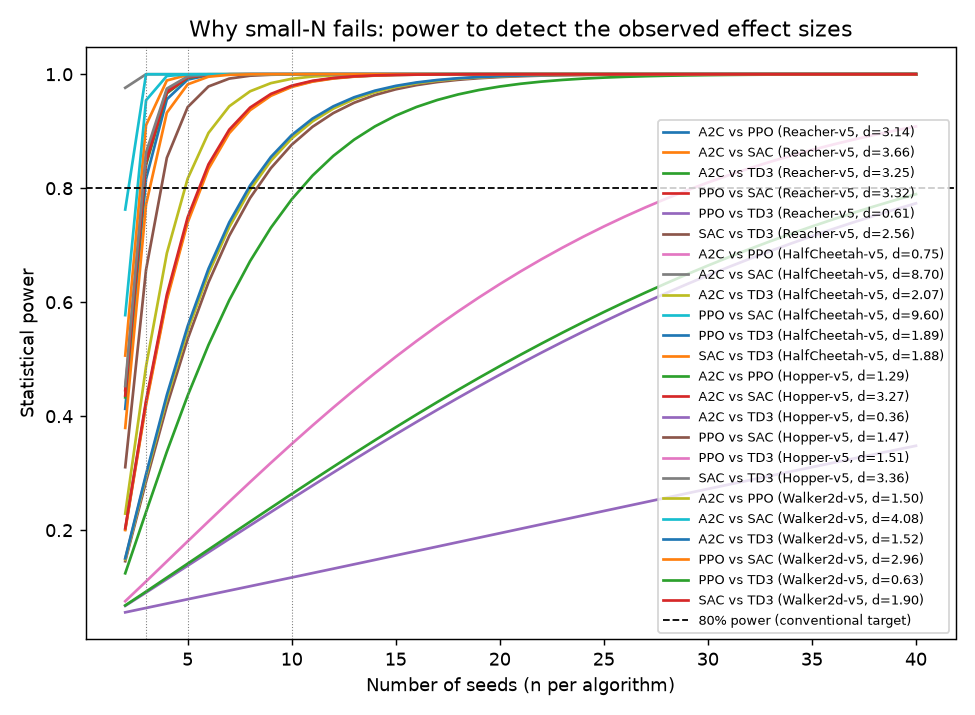
\includegraphics[width=\linewidth]{../figures/power_curves_PILOT4.png}
  \caption{Statistical power to detect each algorithm pair's observed effect size, as a function
  of seed count. Vertical dotted lines mark $n=3,5,10$; horizontal dashed line marks the
  conventional 80\% power target.}
  \label{fig:power}
\end{figure}

\begin{table}[t]
\centering
\footnotesize
\caption{Observed effect sizes (Cohen's $d$) and the statistical power available at conventional small seed counts, with the seed count needed for 80\% power.}
\label{tab:power}
\begin{tabular}{llrrrrr}
\toprule
Env. & Pair & $d$ & $n{=}3$ & $n{=}5$ & $n{=}10$ & $n_{80\%}$ \\
\midrule
Reacher-v5 & A2C vs PPO & 3.14 & 0.82 & 0.99 & 1.00 & 3 \\
Reacher-v5 & A2C vs SAC & 3.66 & 0.91 & 1.00 & 1.00 & 3 \\
Reacher-v5 & A2C vs TD3 & 3.25 & 0.84 & 0.99 & 1.00 & 3 \\
Reacher-v5 & PPO vs SAC & 3.32 & 0.85 & 1.00 & 1.00 & 3 \\
Reacher-v5 & PPO vs TD3 & 0.61 & 0.09 & 0.14 & 0.26 & 43 \\
Reacher-v5 & SAC vs TD3 & 2.56 & 0.66 & 0.94 & 1.00 & 4 \\
HalfCheetah-v5 & A2C vs PPO & 0.75 & 0.11 & 0.18 & 0.35 & 30 \\
HalfCheetah-v5 & A2C vs SAC & 8.70 & 1.00 & 1.00 & 1.00 & 2 \\
HalfCheetah-v5 & A2C vs TD3 & 2.07 & 0.49 & 0.82 & 0.99 & 5 \\
HalfCheetah-v5 & PPO vs SAC & 9.60 & 1.00 & 1.00 & 1.00 & 3 \\
HalfCheetah-v5 & PPO vs TD3 & 1.89 & 0.42 & 0.74 & 0.98 & 6 \\
HalfCheetah-v5 & SAC vs TD3 & 1.88 & 0.42 & 0.74 & 0.98 & 6 \\
Hopper-v5 & A2C vs PPO & 1.29 & 0.23 & 0.44 & 0.78 & 11 \\
Hopper-v5 & A2C vs SAC & 3.27 & 0.84 & 0.99 & 1.00 & 3 \\
Hopper-v5 & A2C vs TD3 & 0.36 & 0.06 & 0.08 & 0.12 & 126 \\
Hopper-v5 & PPO vs SAC & 1.47 & 0.29 & 0.54 & 0.88 & 9 \\
Hopper-v5 & PPO vs TD3 & 1.51 & 0.29 & 0.55 & 0.89 & 9 \\
Hopper-v5 & SAC vs TD3 & 3.36 & 0.86 & 1.00 & 1.00 & 3 \\
Walker2d-v5 & A2C vs PPO & 1.50 & 0.29 & 0.55 & 0.89 & 9 \\
Walker2d-v5 & A2C vs SAC & 4.08 & 0.95 & 1.00 & 1.00 & 3 \\
Walker2d-v5 & A2C vs TD3 & 1.52 & 0.30 & 0.56 & 0.89 & 8 \\
Walker2d-v5 & PPO vs SAC & 2.96 & 0.77 & 0.98 & 1.00 & 4 \\
Walker2d-v5 & PPO vs TD3 & 0.63 & 0.09 & 0.14 & 0.26 & 42 \\
Walker2d-v5 & SAC vs TD3 & 1.90 & 0.43 & 0.75 & 0.98 & 6 \\
\bottomrule
\end{tabular}
\end{table}

\subsection{A Practical Seed-Count Guide}
\label{sec:seed_guide}

The effect sizes above are specific to our four algorithms and four tasks, but the underlying
power calculation is not. Table~\ref{tab:seed_guide} generalizes it into a lookup table usable by
any author or reviewer, independent of algorithm or environment: compute the observed (or
pilot-estimated) Cohen's $d$ for the comparison in question, find the nearest row at or above it,
and read off the minimum seed count for conventional 80\% power (or the more conservative 90\%).
For example, an author who observes $d=0.5$, a conventionally ``medium'' effect, needs at least 64
seeds, not three or five, to have even an 80\% chance of detecting it with a two-sample $t$-test at
$\alpha=0.05$; a reviewer evaluating a three-seed study making a $d\approx0.5$ claim can point to
this table directly rather than reconstructing the power calculation from scratch. The table
includes two of our own observed effect sizes from Table~\ref{tab:power} for concrete anchoring,
including our smallest ($d=0.36$, Hopper-v5, requiring 126 seeds), which shows just how far a
genuinely small but real effect can push the required sample size beyond what any of the
conventional textbook effect-size bands would suggest.

\begin{table}[t]
\centering
\footnotesize
\caption{Practical seed-count guide: minimum seeds for 80\%/90\% power to detect a two-sample effect of a given size $|d|$ (Welch's $t$-test, $\alpha{=}0.05$). Find your own observed $|d|$, round up to the nearest row.}
\label{tab:seed_guide}
\begin{tabular}{lrrl}
\toprule
$|d|$ & $n_{80\%}$ & $n_{90\%}$ & Note \\
\midrule
0.20 & 393 & 526 & small (Cohen) \\
0.30 & 176 & 234 &  \\
0.35 & 126 & 168 & observed: A2C vs.\ TD3, Hopper \\
0.50 & 64 & 86 & medium (Cohen) \\
0.61 & 44 & 58 & observed: PPO vs.\ TD3, Reacher \\
0.75 & 29 & 39 & observed: A2C vs.\ PPO, HalfCheetah \\
0.80 & 26 & 34 & large (Cohen) \\
1.00 & 17 & 23 &  \\
1.20 & 12 & 16 &  \\
1.50 & 9 & 11 &  \\
2.00 & 6 & 7 &  \\
\bottomrule
\end{tabular}
\end{table}

\section{Discussion}

Our results support five concrete, actionable recommendations for robot-control RL research, in
the spirit of but more directly quantified than \cite{henderson2018deep} and
\cite{colas2018many}.

First, when an algorithmic improvement's effect size is genuinely large (as with most of the
algorithm gaps we observe here), a small seed count usually still finds it, but not reliably: even
our largest observed effect sizes leave a non-trivial disagreement rate at $k=3$
(Table~\ref{tab:smalln}), meaning that a lucky or unlucky draw of three seeds can flip a
publication's headline claim. Reporting five or more seeds sharply reduces, but does not
eliminate, this risk.

Second, when an effect is modest, no seed count in the range typically used in the literature is
likely to resolve it (Table~\ref{tab:power}), and this is not a one-environment quirk: we observe
it independently on Reacher-v5, Hopper-v5, and Walker2d-v5. In the most extreme case we observe,
resolving the effect with conventional 80\% power would need an estimated 126 seeds. A ``no
significant difference'' finding under these conditions should be reported as inconclusive due to
insufficient power, not as evidence of equivalence, and Walker2d-v5's PPO-vs-TD3 comparison shows
this is not merely hypothetical: even our own full twenty-seed sample stays inconclusive on it. This
is arguably the paper's deepest lesson: rigor does not guarantee a verdict, and an honest
``unresolved at this sample size'' beats forcing a call either way.

Third, this is not a purely hypothetical risk in the other direction either: at our full sample
size of twenty seeds, a conventional Welch's $t$-test already missed two real effects (PPO vs.\
TD3 on Reacher-v5, A2C vs.\ TD3 on Hopper-v5) that our rigorous bootstrap method correctly
detected, on two independently trained environments. A seed count several times larger than what
most comparative RL papers report was still not enough to make the naive test reliable for either
comparison.

Fourth, both missed effects share the same mechanism: an off-policy algorithm (TD3 in both cases)
whose seed-to-seed variance is inflated by occasional training failures, from a single low-outlier
run to outright bimodal collapse, breaks the normality assumption behind mean-based tests without
breaking a rank-based one. When comparing an algorithm known to exhibit such instability, a
Mann-Whitney-style rank test is not just more statistically efficient in the abstract, it is
specifically more robust to exactly the failure mode that algorithm is prone to.

Fifth, multiple-comparison correction, while it did not change any conclusion in our particular
dataset (Table~\ref{tab:pairwise}), is an independent source of inflated significance claims
whenever more than one pairwise comparison is run, and costs nothing to apply.

\section{Limitations and Future Work}

This audit covers four algorithms, four environments, and a single training budget (200{,}000
timesteps); the disagreement rates we report are properties of \emph{these} effect sizes and
should not be read as universal constants. All four environments are MuJoCo continuous-control
locomotion or reaching tasks with dense rewards and low-dimensional proprioceptive observations; we
have not tested whether the same pattern holds for manipulation tasks, sparse-reward settings,
vision-based observations, or discrete-action domains, and a natural extension, enabled directly by
our released pipeline, is to repeat this analysis on such tasks, with more algorithms and longer
training budgets, to test how far the qualitative pattern generalizes. We also fixed all
hyperparameters to Stable-Baselines3 defaults; a tuned comparison could show different effect sizes
and therefore different reliability profiles. Finally, our small-$N$ analysis draws sub-studies
from a pool of twenty seeds; an even larger pool would let us test whether the two persistent
disagreement rates of Section~\ref{sec:smalln} eventually reach zero, resolve the still-inconclusive
Walker2d-v5 case, and probe sparser regimes (e.g., $k=1,2$).

\section{Conclusion}

We provide a direct, quantitative answer to a question implicit in years of reproducibility
concerns about deep RL: given the seed budgets robot-control papers typically report, how often
would their conclusions have differed from a much larger, statistically rigorous study of the same
comparison? For the algorithms and tasks studied here, the answer depends entirely on effect size,
and this holds consistently across four independently trained environments, not just one. For
large effects, disagreement is a real concern at three seeds but becomes negligible by five to ten.
For modest effects, the risk is far more persistent: two of our twenty-four comparisons remain
unreliable even at nineteen of twenty seeds (one of them still wrong 95\% of the time), a third
remains inconclusive under both methods even at our full twenty-seed budget, and a statistical
power analysis confirms this persistence follows directly from the underlying effect sizes rather
than any artifact of the naive test, with our hardest case requiring an estimated 126 seeds for
conventional 80\% power. Even our full twenty-seed sample produced two comparisons, on two
different environments, where a conventional significance test missed a real effect our rigorous
method correctly detected, and in both cases the same mechanism was responsible: TD3's
seed-to-seed variance, inflated by occasional training failures, breaks a mean-based test without
breaking a rank-based one. We also derive a general, effect-size-indexed seed-count table for
authors and reviewers to apply directly. We release our full pipeline so this audit can be
extended to other algorithms, tasks, and seed budgets.

\section*{Code and Data Availability}
All training, analysis, and figure-generation code, together with the raw per-seed evaluation
results, will be released publicly upon publication. A link is withheld from this submission to
preserve double-anonymous review; an anonymized copy can be made available to reviewers on
request through the venue's review system.

{\footnotesize
\bibliographystyle{IEEEtran}
\bibliography{refs}
}

\end{document}
